%package list
\documentclass{article}
\usepackage[top=3cm, bottom=3cm, outer=3cm, inner=3cm]{geometry}
\usepackage{multicol}
\usepackage{graphicx}
\usepackage{url}
%\usepackage{cite}
\usepackage{hyperref}
\usepackage{array}
%\usepackage{multicol}
\newcolumntype{x}[1]{>{\centering\arraybackslash\hspace{0pt}}p{#1}}
\usepackage{natbib}
\usepackage{pdfpages}
\usepackage{multirow}
\usepackage[normalem]{ulem}
\useunder{\uline}{\ul}{}
\usepackage{svg}
\usepackage{xcolor}
\usepackage{listings}
\lstdefinestyle{ascii-tree}{
    literate={├}{|}1 {─}{--}1 {└}{+}1 
  }
\lstset{basicstyle=\ttfamily,
  showstringspaces=false,
  commentstyle=\color{red},
  keywordstyle=\color{blue}
}
%\usepackage{booktabs}
\usepackage{caption}
\usepackage{subcaption}
\usepackage{float}
\usepackage{array}

\newcolumntype{M}[1]{>{\centering\arraybackslash}m{#1}}
\newcolumntype{N}{@{}m{0pt}@{}}


%%%%%%%%%%%%%%%%%%%%%%%%%%%%%%%%%%%%%%%%%%%%%%%%%%%%%%%%%%%%%%%%%%%%%%%%%%%%
%%%%%%%%%%%%%%%%%%%%%%%%%%%%%%%%%%%%%%%%%%%%%%%%%%%%%%%%%%%%%%%%%%%%%%%%%%%%
\newcommand{\itemEmail}{schirinosne@unsa.edu.pe / gsotocco@unsa.edu.pe}
\newcommand{\itemStudent}{Sebastian Arley Chirinos Negrón/ Gabriel Eduardo Soto Ccoya}
\newcommand{\itemCourse}{Estructura de datos y Algoritmos}
\newcommand{\itemCourseCode}{1702124}
\newcommand{\itemSemester}{I}
\newcommand{\itemUniversity}{Universidad Nacional de San Agustín de Arequipa}
\newcommand{\itemFaculty}{Facultad de Ingeniería de Producción y Servicios}
\newcommand{\itemDepartment}{Departamento Académico de Ingeniería de Sistemas e Informática}
\newcommand{\itemSchool}{Escuela Profesional de Ingeniería de Sistemas}
\newcommand{\itemAcademic}{2023 - A}
\newcommand{\itemInput}{26 Junio 2023}
\newcommand{\itemOutput}{3 Julio 2023
}
\newcommand{\itemPracticeNumber}{08}
\newcommand{\itemTheme}{Django Rest Framework}
%%%%%%%%%%%%%%%%%%%%%%%%%%%%%%%%%%%%%%%%%%%%%%%%%%%%%%%%%%%%%%%%%%%%%%%%%%%%
%%%%%%%%%%%%%%%%%%%%%%%%%%%%%%%%%%%%%%%%%%%%%%%%%%%%%%%%%%%%%%%%%%%%%%%%%%%%

\usepackage[english,spanish]{babel}
\usepackage[utf8]{inputenc}
\AtBeginDocument{\selectlanguage{spanish}}
\renewcommand{\figurename}{Figura}
\renewcommand{\refname}{Referencias}
\renewcommand{\tablename}{Tabla} %esto no funciona cuando se usa babel
\AtBeginDocument{%
	\renewcommand\tablename{Tabla}
}

\usepackage{fancyhdr}
\pagestyle{fancy}
\fancyhf{}
\setlength{\headheight}{30pt}
\renewcommand{\headrulewidth}{1pt}
\renewcommand{\footrulewidth}{1pt}
\fancyhead[L]{\raisebox{-0.2\height}{
\includegraphics[width=3cm]{img/logo_episunsa.png}}}
\fancyhead[C]{\fontsize{7}{7}\selectfont	\itemUniversity \\ \itemFaculty \\ \itemDepartment \\ \itemSchool \\ \textbf{\itemCourse}}
\fancyhead[R]{\raisebox{-0.2\height}{
\includegraphics[width=1.2cm]{img/logo_abet}}}
\fancyfoot[L]{Sebastian Chirinos/Gabriel Soto}
\fancyfoot[C]{\itemCourse}
\fancyfoot[R]{Página \thepage}

% para el codigo fuente
\usepackage{listings}
\usepackage{color, colortbl}
\definecolor{dkgreen}{rgb}{0,0.6,0}
\definecolor{gray}{rgb}{0.5,0.5,0.5}
\definecolor{mauve}{rgb}{0.58,0,0.82}
\definecolor{codebackground}{rgb}{72, 0.95, 0.92}
\definecolor{tablebackground}{rgb}{0.8, 0, 0}

\lstset{frame=tb,
	language=bash,
	aboveskip=3mm,
	belowskip=3mm,
	showstringspaces=false,
	columns=flexible,
	basicstyle={\small\ttfamily},
	numbers=none,
	numberstyle=\tiny\color{gray},
	keywordstyle=\color{blue},
	commentstyle=\color{dkgreen},
	stringstyle=\color{mauve},
	breaklines=true,
	breakatwhitespace=true,
	tabsize=3,
	backgroundcolor= \color{codebackground},
}

\begin{document}
	
	\vspace*{10px}
	
	\begin{center}	
		\fontsize{17}{17} \textbf{ Informe de Laboratorio \itemPracticeNumber}
	\end{center}
	\centerline{\textbf{\Large Tema: \itemTheme}}
	%\vspace*{0.5cm}	

	\begin{flushright}
		\begin{tabular}{|M{2.5cm}|N|}
			\hline 
			\rowcolor{tablebackground}
			\color{white} \textbf{Nota}  \\
			\hline 
			     \\[30pt]
			\hline 			
		\end{tabular}
	\end{flushright}	

	\begin{table}[H]
		\begin{tabular}{|x{4.7cm}|x{4.8cm}|x{4.8cm}|}
			\hline 
			\rowcolor{tablebackground}
			\color{white} \textbf{Estudiante} & \color{white}\textbf{Escuela}  & \color{white}\textbf{Asignatura}   \\
			\hline 
			{\itemStudent \par \itemEmail} & \itemSchool & {\itemCourse \par Semestre: \itemSemester \par Código: \itemCourseCode}     \\
			\hline 			
		\end{tabular}
	\end{table}		
	
	\begin{table}[H]
		\begin{tabular}{|x{4.7cm}|x{4.8cm}|x{4.8cm}|}
			\hline 
			\rowcolor{tablebackground}
			\color{white}\textbf{Laboratorio} & \color{white}\textbf{Tema}  & \color{white}\textbf{Duración}   \\
			\hline 
			\itemPracticeNumber & \itemTheme & 04 horas   \\
			\hline 
		\end{tabular}
	\end{table}
	
	\begin{table}[H]
		\begin{tabular}{|x{4.7cm}|x{4.8cm}|x{4.8cm}|}
			\hline 
			\rowcolor{tablebackground}
			\color{white}\textbf{Semestre académico} & \color{white}\textbf{Fecha de inicio}  & \color{white}\textbf{Fecha de entrega}   \\
			\hline 
			\itemAcademic & \itemInput &  \itemOutput  \\
			\hline 
		\end{tabular}
	\end{table}
	
	\section{Tarea}
	\begin{itemize}
		\item Introducción
En este informe, se presenta la implementación de B+.

	\end{itemize}	
		

	\section{URL de Repositorio Github}
	\begin{itemize}
		\item URL para el laboratorio 04 en el Repositorio GitHub.
		\item \url{ https://github.com/GabSoto/Pweb02_Lab08}
	\end{itemize}
	
	\section{Tarea}

	\subsection{Django Rest Framework}
	\begin{itemize}
		
	\item En sus grupos de trabajo correspondientes. Elabore un servicio web que tenga un CRUD con el uso de este framework.

	En este párrafo, se solicita a los grupos de trabajo que elaboren un servicio web que implemente las operaciones CRUD (Create, Read, Update, Delete) utilizando un framework específico. El CRUD es una operación básica que se refiere a las acciones de crear, leer, actualizar y eliminar datos en una base de datos o sistema de almacenamiento. El servicio web debe ser capaz de realizar estas operaciones para gestionar los datos de manera eficiente.

	\item Create - POST
	\item Read - GET
	\item Update - PUT
	\item Delete - DELETE

	\item Aquí se describen los métodos HTTP asociados con cada una de las operaciones CRUD. Estos métodos son estándares en la comunicación REST (Representational State Transfer) y son utilizados para realizar diferentes acciones sobre los recursos en un servicio web. Por ejemplo, para crear un nuevo recurso, se utiliza el método POST; para leer o recuperar un recurso, se utiliza el método GET; para actualizar un recurso existente, se utiliza el método PUT; y para eliminar un recurso, se utiliza el método DELETE.
	\item Centrarse en el Core business de su aplicación web. Los más importante y necesario que esté disponible a través de un servicio web.En esta parte del texto, se destaca la importancia de centrarse en el "Core business" de la aplicación web al diseñar el servicio web. El término "Core business" se refiere a la parte central o núcleo de la aplicación, que contiene las funcionalidades más importantes y necesarias para el funcionamiento principal de la aplicación. Al implementar el servicio web, es esencial priorizar las funcionalidades principales y asegurarse de que estén disponibles a través del servicio web para que puedan ser utilizadas por los clientes y usuarios.
	\end{itemize}

	%%%%%%%%%%%%%%%%%%%%%%%%%%%%%%%%%%%%%%%%%%%%%%%%%%%%%%%%%%%%%%%%%%%%%%%%%%%%%%%%%%%%%%%%%%%%%

	\subsection{models}
	\begin{itemize}
		
		\item Este código define un modelo de Django, que es una clase de Python que representa una tabla de base de datos. Django es un marco de trabajo web que te permite construir aplicaciones web utilizando el lenguaje de programación Python, y proporciona un sistema de mapeo objeto-relacional (ORM) para interactuar con bases de datos.

		\item Vamos a revisar el código paso a paso:
		
		\item from django.db import models: Esta línea importa los módulos necesarios del módulo de base de datos de Django. Esto te permite usar la funcionalidad de los modelos de Django para definir la estructura de la tabla de base de datos.
		
		\item class data user models.Model:: Esta línea define un modelo de Django llamado data user. Es una subclase de models.Model, lo que significa que hereda todas las funcionalidades de la clase de modelo base de Django. Al heredar de models.Model, esta clase tiene todas las funcionalidades de un modelo de Django.
		

		\item Dentro de la clase data user, defines varios campos que representan las columnas en la tabla de base de datos:
		
		\item dni  Esto define un campo de caracteres (una cadena) con una longitud máxima de 8 caracteres. Representa el "dni" (número de documento) del usuario.
		
		\item nombre = models.CharField Esto define un campo de caracteres con una longitud máxima de 100 caracteres. Representa el "nombre" del usuario.
		
		\item apellidos = models.CharField Esto define un campo de caracteres con una longitud máxima de 100 caracteres. Representa los "apellidos" del usuario.
		
		\item contraseña = models.CharField: Esto define un campo de caracteres con una longitud máxima de 20 caracteres. Representa la "contraseña" del usuario.
		
		\item Cada campo corresponde a una columna en la tabla de base de datos y tiene un tipo de dato específico asociado.
		
		\item def str(self):: Este método está definido para controlar cómo se representan las instancias de la clase data user como cadenas. Cuando imprimes una instancia de esta clase o la muestras en la interfaz de administración de Django, mostrará el nombre y dni del usuario.
		
		\item Por ejemplo, si tienes una instancia de data user con nombre configurado como "John" y dni configurado como "12345678", al llamar a print(instancia) o mostrarla en la interfaz de administración, se mostrará: "John dni: 12345678".
		
		\item En resumen, este código define un modelo de Django llamado data user, que representa una tabla de base de datos con columnas para "dni", "nombre", "apellidos" y "contraseña". El método str está implementado para proporcionar una representación legible para humanos de las instancias de data user. Este modelo se puede utilizar para almacenar y recuperar datos relacionados con usuarios en una aplicación web de Django.
	\end{itemize}	
	\lstinputlisting[language=Python, caption={models.py},numbers=left,]{src/models.py}	

	\subsection{forms}
	\begin{itemize}	
		
			\item login\_form(forms.Form): Esta clase representa un formulario de inicio de sesión. Contiene dos campos: "dni" y "password", donde los usuarios ingresarán su número de documento (dni) y contraseña para iniciar sesión.
			\item dni = forms.CharField(label="", max\_length=8, widget=forms.TextInput(attrs={'placeholder': 'Ingresa tu DNI', 'data-lpignore': 'true'})): Este campo es un campo de texto (CharField) que tiene una etiqueta vacía (label="") para que no se muestre ninguna etiqueta al usuario. Tiene una longitud máxima de 8 caracteres (max\_length=8). El widget asociado es un TextInput, que muestra un campo de entrada de texto en el formulario. Además, se le asigna un atributo placeholder con el valor "Ingresa tu DNI", que es un texto de ejemplo que se muestra en el campo antes de que el usuario ingrese su DNI. También tiene el atributo data-lpignore con valor "true", que podría estar relacionado con algún script de terceros o complemento utilizado en la página.
			\item password = forms.CharField(label="", widget=forms.PasswordInput(attrs={'placeholder': 'Introduce tu contraseña', 'data-lpignore': 'true'})): Este campo es similar al anterior, pero es para ingresar la contraseña. Tiene un widget de PasswordInput, que oculta el texto ingresado para proteger la privacidad de la contraseña. También tiene un atributo placeholder con el valor "Introduce tu contraseña", que muestra un texto de ejemplo en el campo. Al igual que el campo anterior, tiene el atributo data-lpignore con valor "true".
			\item register: Esta clase representa un formulario de registro. Contiene cuatro campos: "dni", "name", "surname" y "password", donde los usuarios ingresarán su número de documento, nombres, apellidos y una contraseña para crear una cuenta.
			\item dni : Este campo es similar al campo "dni" en el formulario de inicio de sesión, pero en este caso, tiene el atributo autocomplete con valor "off". Esto indica al navegador que no debe autocompletar este campo, lo cual es útil para campos sensibles como el número de documento.
			\item name : Este campo es para ingresar los nombres del usuario. Tiene un atributo autocomplete con valor "off" para evitar el autocompletado del navegador.
			\item surname: Este campo es para ingresar los apellidos del usuario. También tiene el atributo autocomplete con valor "off".
			\item password: Este campo es para crear una contraseña para la cuenta. Tiene un widget de PasswordInput, y también tiene el atributo autocomplete con valor "off" para proteger la privacidad de la contraseña.
			\item En resumen, este código define dos clases de formularios de Django: login form y register form. Estos formularios se pueden utilizar para crear páginas de inicio de sesión y registro en una aplicación web, y están diseñados para recopilar y validar información como el número de documento, nombres, apellidos y contraseñas de los usuarios. Los atributos placeholder y autocomplete se utilizan para proporcionar sugerencias y mejorar la experiencia del usuario al interactuar con los formularios.
			
	\end{itemize}	
	
	\lstinputlisting[language=Python, caption={forms.py},numbers=left,]{src/forms.py}	

%%%%%%%%%%%%%%%%%%%%%%%%%%%%%%%%%%%%%%%%%%%%%%%%%%%%%%%%%%%%%%%%%%%%%%%%%%%%%%%%%%%%%%%%%%%%%%%%%%%%%%%%%%
%%%%%%%%%%%%%%%%%%%%%%%%%%%%%%%%%%%%%%%%%%%%%%%%%%%%%%%%%%%%%%%%%%%%%%%%%%%%%%%%%%%%%%%%%%%%%
\subsection{view}
\begin{itemize}	
	\item Este código es parte de un proyecto Django que contiene algunas vistas y funciones relacionadas con el inicio de sesión y el registro de usuarios. A continuación, te explico las funciones y vistas presentes en el código:
	\item showHome(request): Esta vista renderiza una plantilla llamada "home.html". Esta función parece ser una página de inicio o página principal del sitio web.

	\item showForm(request): Esta vista renderiza una plantilla llamada "login.html" y pasa el formulario login\_form como contexto. Esta función maneja el proceso de inicio de sesión de los usuarios.
	
	\item showRegister(request): Esta vista maneja el proceso de registro de nuevos usuarios. Si la solicitud es una petición "GET", renderiza la plantilla "register.html" y pasa el formulario register\_form como contexto. Si la solicitud es una petición "POST", extrae los datos ingresados por el usuario (dni, nombre, apellidos y contraseña) y realiza algunas verificaciones.
	
	\item isValid(req, api): Esta función auxiliar recibe dos cadenas de texto como entrada (req y api) y realiza una comparación entre ellas después de eliminar espacios y convertir ambas cadenas a mayúsculas. Se utiliza para verificar si el nombre y apellidos ingresados por el usuario coinciden con los datos obtenidos de una API externa que proporciona información sobre el número de documento (DNI) ingresado.
	
	\item El código hace uso de algunos módulos y clases de Django, como render, redirect, HttpResponse, messages, data\_user, login\_form y register\_form. También utiliza la biblioteca urlopen para realizar solicitudes a una API externa y la biblioteca json para manejar las respuestas en formato JSON.
	
	\item Sin el contexto completo del proyecto y las plantillas asociadas, es posible que no se pueda obtener una imagen completa de todas las funcionalidades y flujos de la aplicación. Pero, en resumen, parece estar implementando un sistema de inicio de sesión y registro de usuarios utilizando formularios de Django y validaciones adicionales a través de una API externa para el DNI.
	
\end{itemize}	
\lstinputlisting[language=Python, caption={views.py},numbers=left,]{src/viewss.py}	

\subsection{quickstart.view}
\begin{itemize}	
	\item Este código muestra dos clases de serializadores utilizando la biblioteca rest framework de Django para manejar la serialización y deserialización de objetos en una API web.
	\item UserSerializer: Esta clase de serializador se utiliza para convertir objetos del modelo User de Django en formato JSON, y viceversa, para su uso en una API web.

\item GroupSerializer: Esta clase de serializador se utiliza para convertir objetos del modelo Group de Django en formato JSON, y viceversa, para su uso en una API web.

\item Para configurar qué campos del modelo se incluirán en la serialización, se utiliza la clase interna Meta, que especifica el modelo que se está serializando (model) y la lista de campos que se deben incluir en el JSON resultante (fields).

\item En el caso del UserSerializer, se incluyen los campos 'url', 'username', 'email' y 'groups' del modelo User, lo que significa que estos campos serán incluidos en el JSON resultante cuando se serialice un objeto User.

\item En el caso del GroupSerializer, se incluyen los campos 'url' y 'name' del modelo Group, lo que significa que estos campos serán incluidos en el JSON resultante cuando se serialice un objeto Group.

\item Estos serializadores son útiles cuando se desea exponer datos de modelos Django como parte de una API web, lo que permite que los clientes realicen solicitudes HTTP para obtener, crear, actualizar y eliminar objetos del modelo a través de la API.

\end{itemize}	
\lstinputlisting[language=Python, caption={views.py},numbers=left,]{src/views.py}	
\subsection{serializer}
\begin{itemize}	
	\item Este código muestra dos clases de vistas basadas en conjuntos (viewsets) para manejar las operaciones CRUD (crear, leer, actualizar y eliminar) en los modelos User y Group de Django utilizando la biblioteca rest framework.
	\item UserViewSet: Esta clase de vista define un conjunto de vistas para el modelo User. Específicamente, permite ver y editar objetos User a través de la API web. La clase hereda de viewsets.ModelViewSet, que proporciona las funcionalidades necesarias para realizar operaciones CRUD.

\item queryset = User.objects.all().order by('-datejoined'): Esto define el conjunto de objetos User que serán accesibles a través de la API. En este caso, se obtienen todos los objetos User y se los ordena por la fecha de unión (date joined) en orden descendente.

\item serializer class = UserSerializer: Esta propiedad define el serializador que se utilizará para convertir los objetos User en formato JSON y viceversa. Utiliza el UserSerializer definido previamente.

\item permission classes = [permissions.IsAuthenticated]: Esta propiedad define las clases de permisos requeridas para acceder a las vistas. En este caso, se requiere que el usuario esté autenticado (IsAuthenticated) para acceder a estas vistas, lo que significa que solo los usuarios autenticados tendrán permiso para ver y editar objetos User.

\item GroupViewSet: Esta clase de vista define un conjunto de vistas para el modelo Group. Permite ver y editar objetos Group a través de la API web. Al igual que UserViewSet, hereda de viewsets.ModelViewSet y proporciona las funcionalidades CRUD necesarias.

\item queryset = Group.objects.all(): Esto define el conjunto de objetos Group que serán accesibles a través de la API. En este caso, se obtienen todos los objetos Group.

\item serializer class = GroupSerializer: Esta propiedad define el serializador que se utilizará para convertir los objetos Group en formato JSON y viceversa. Utiliza el GroupSerializer definido previamente.

\item permission classes = [permissions.IsAuthenticated]: Al igual que en UserViewSet, se requiere que el usuario esté autenticado para acceder a estas vistas de grupos.

\item Estas vistas basadas en conjuntos simplifican en gran medida la creación de una API REST para los modelos User y Group. Con estas configuraciones, las rutas y puntos finales de la API serán generados automáticamente, permitiendo realizar operaciones CRUD en los objetos User y Group a través de los métodos HTTP correspondientes (GET, POST, PUT, DELETE, etc.). Además, se asegura de que solo los usuarios autenticados puedan acceder a estas vistas.

	
\end{itemize}	
\lstinputlisting[language=Python, caption={serializers.py},numbers=left,]{src/serializers.py}	


\subsection{urls}
\begin{itemize}	
	\item Este fragmento de código muestra cómo se configuran las URLs (rutas) para el enrutamiento en una aplicación Django. La variable \texttt{urlpatterns} es una lista de rutas que mapean las URL de la aplicación a las vistas correspondientes que se deben mostrar cuando se accede a esas rutas.
	\item \texttt{from django.urls import path}: Esta línea importa la función \texttt{path} del módulo \texttt{django.urls}, que se utiliza para definir rutas (URL) dentro de la aplicación Django.

\item \texttt{from . import views}: Esta línea importa las vistas definidas en el archivo \texttt{views.py} del directorio actual (\texttt{.}). Las vistas son funciones que manejan las solicitudes HTTP y devuelven las respuestas apropiadas.

\item \texttt{urlpatterns}: Esta es una lista que contiene todas las rutas definidas para la aplicación Django.

\item \texttt{path("login/", views.showForm, name="showForm")}: Esta línea define una ruta para la página de inicio de sesión. Cuando un usuario accede a la ruta \texttt{/login/} en la aplicación, la función \texttt{showForm} dentro del archivo \texttt{views.py} será llamada para manejar la solicitud. El parámetro \texttt{name="showForm"} se utiliza para darle un nombre a esta ruta, lo cual es útil para referirse a ella de manera más sencilla en otras partes del código.


\item \texttt{path("home/", views.showHome, name="showHome")}: Esta línea define una ruta para la página principal del sitio web. Cuando un usuario accede a la ruta \texttt{/home/}, la función \texttt{showHome} dentro del archivo \texttt{views.py} será llamada para manejar la solicitud.

\item En resumen, el fragmento de código configura las rutas de la aplicación Django de acuerdo con las funciones de vistas definidas en \texttt{views.py}. Cuando un usuario ingrese a una ruta específica en el navegador, la función de vista correspondiente se ejecutará para mostrar la página asociada a esa ruta. Estas rutas son útiles para navegar y acceder a diferentes páginas y funcionalidades dentro de la aplicación web.

\end{itemize}	
\lstinputlisting[language=Python, caption={urls.py},numbers=left,]{src/urls.py}	

\subsection{Capturas del trabajo}
	\begin{itemize}	
		\item 
	\end{itemize}	
	
	\begin{figure}[H]
		\centering
		
\includegraphics[width=0.7\textwidth,keepaspectratio]{img/1.png}
		%\includesvg{img/automata.svg}
		%\label{img:mot2}
		%\caption{Product backlog.}
	\end{figure}
	\begin{figure}[H]
		\centering
		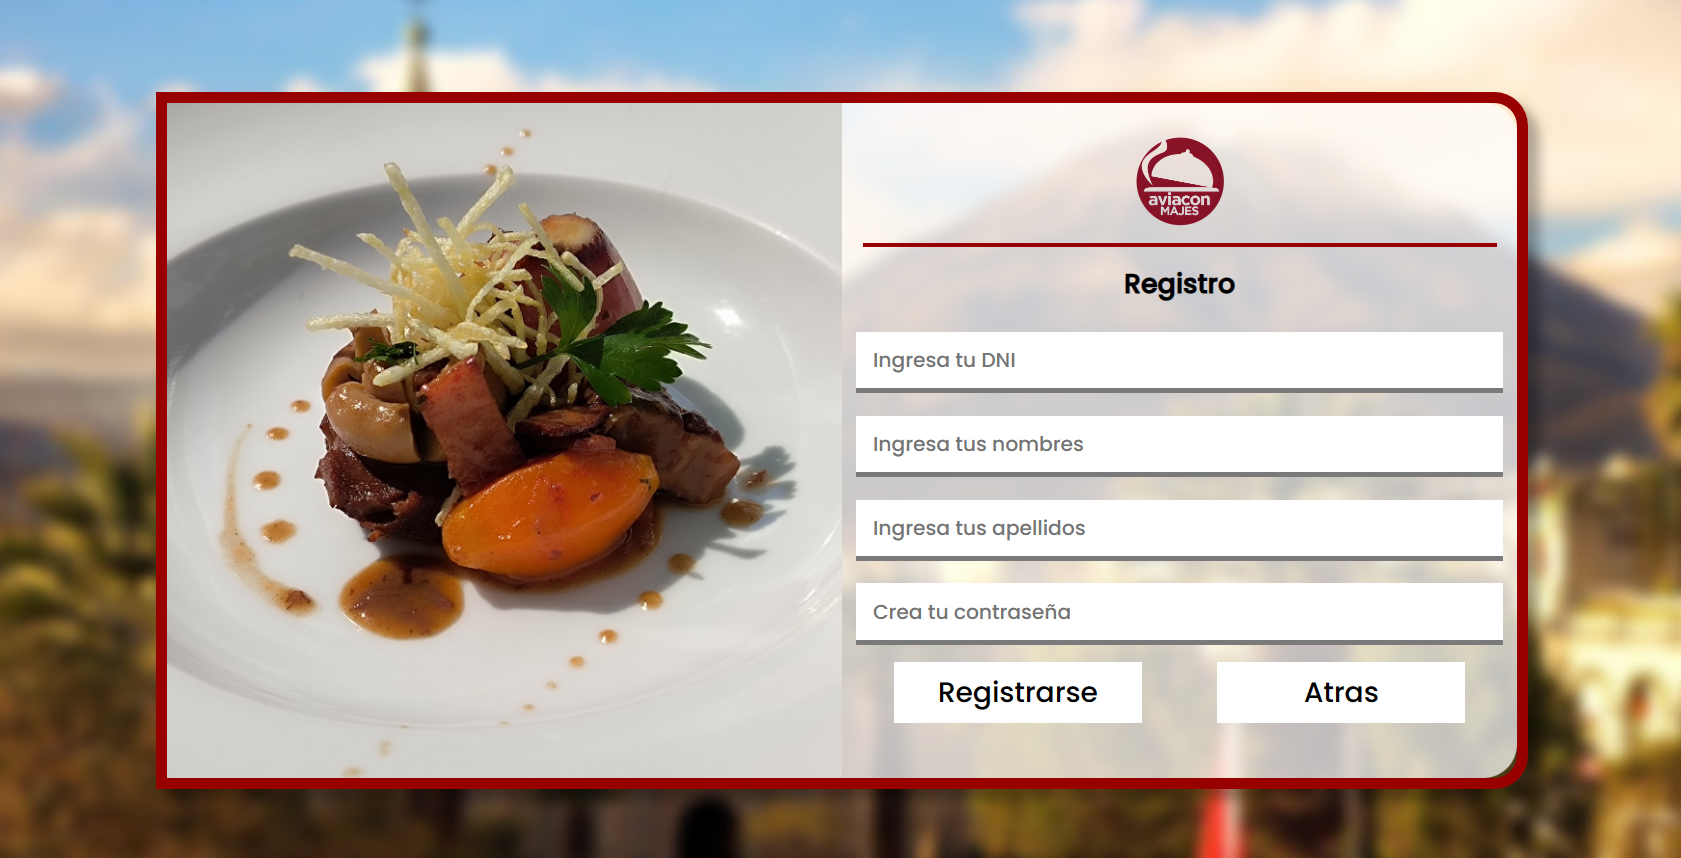
\includegraphics[width=0.7\textwidth,keepaspectratio]{img/2.png}
		%\includesvg{img/automata.svg}
		%\label{img:mot2}
		%\caption{Product backlog.}
	\end{figure}
	\begin{figure}[H]
		\centering
		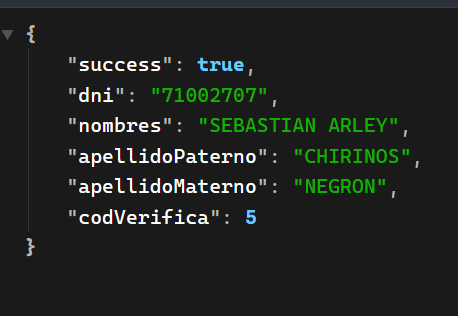
\includegraphics[width=0.7\textwidth,keepaspectratio]{img/4.png}
		%\includesvg{img/automata.svg}
		%\label{img:mot2}
		%\caption{Product backlog.}
	\end{figure}
	\begin{figure}[H]
		\centering
		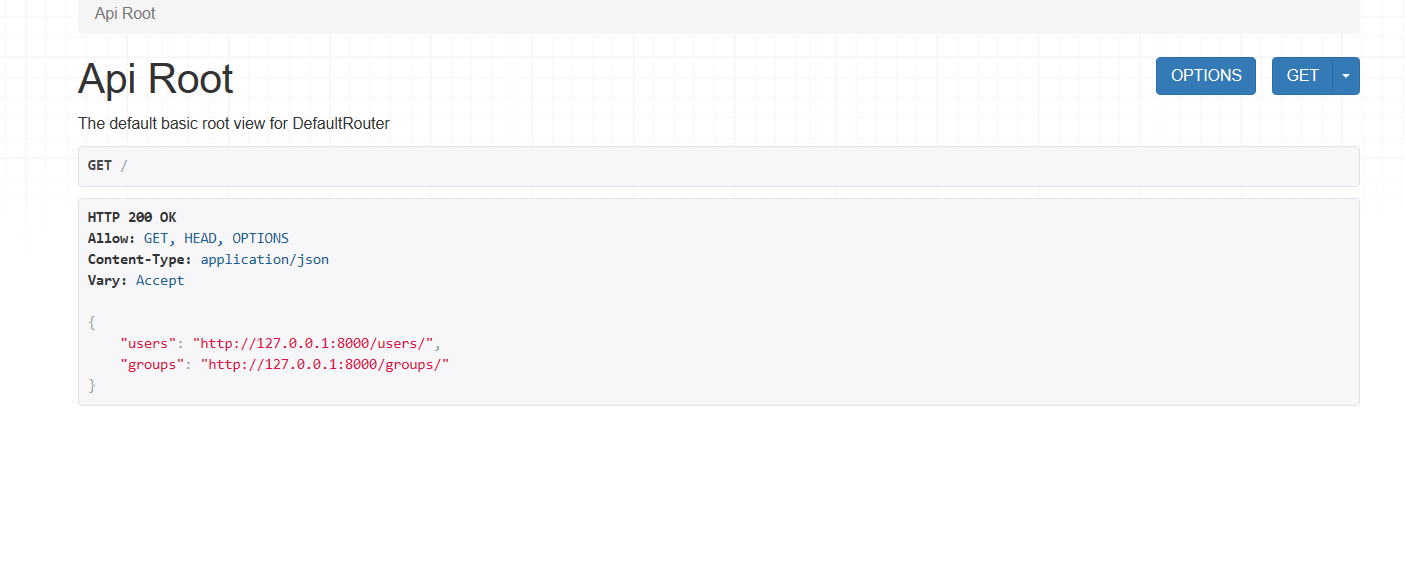
\includegraphics[width=0.7\textwidth,keepaspectratio]{img/3.png}
		%\includesvg{img/automata.svg}
		%\label{img:mot2}
		%\caption{Product backlog.}
	\end{figure}


%%%%%%%%%%%%%%%%%%%%%%%%%%%%%%%%%%%%%%%%%%%%%%%%%%%%%%%%%%%%%%%%%%%%%%%%%%%%%%%%%%%%%%%%%%%%%%%%%%



%%%%%%%%%%%%%%%%%%%%%%%%%%%%%%%%%%%%%%%%%%%%%%%%%%%%%%%%%%%%%%%%%%%%%%%%%%%%%%%%%%


	\subsection{Commits del trabajo}
	\begin{itemize}	
		\item Acá estan algunos de los commits mas importantes en este trabajo:
	\end{itemize}	
	
	\begin{figure}[H]
		\centering
		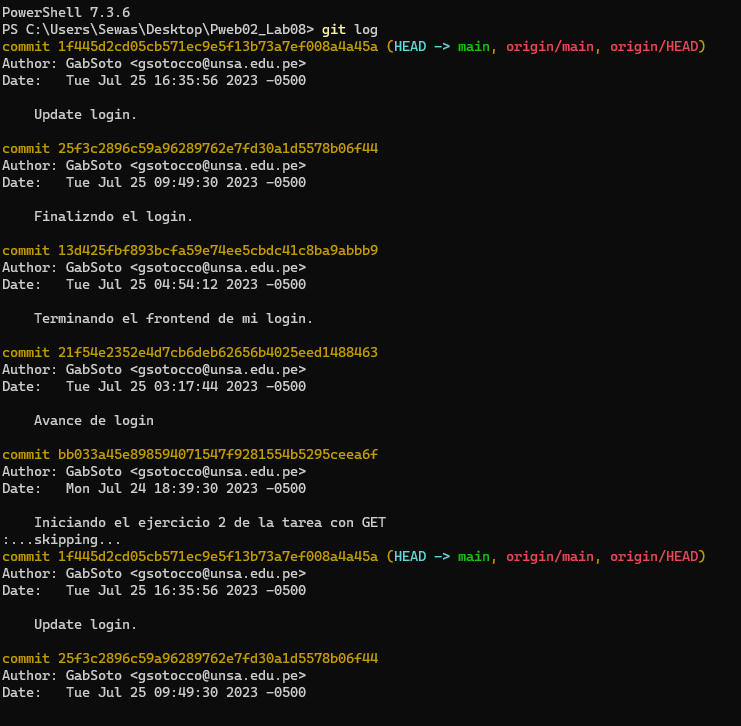
\includegraphics[width=0.7\textwidth,keepaspectratio]{img/Commits.png}
		%\includesvg{img/automata.svg}
		%\label{img:mot2}
		%\caption{Product backlog.}
	\end{figure}


%%%%%%%%%%%%%%%%%%%%%%%%%%%%%%%%%%%%%%%%%%%%%%%%%%%%%%%%%%%%%%%%%%%%%%%%%%%%%%%%%%
	
		
	\subsection{Estructura de laboratorio 08}
	\begin{itemize}	
		\item El contenido que se entrega en este laboratorio es el siguiente:
	\end{itemize}
	
\begin{lstlisting}[style=ascii-tree]
lab08/
|   .gitignore
|	ApiDjangoProject

\---latex
    |	EDA_lab08.pdf
    |   EDA_lab08.tex
    |
    +---img
    |       Commits.png
    |       1.png
    |       2.png
    |       3.png
    |       4.png
    |       logo_abet.png
    |       logo_episunsa.png
    |       logo_unsa.jpg
    |
    \---src
	|		views.py
	|		models.py
	|		forms.py
	|		urls.py
\end{lstlisting}    


	\section{\textcolor{red}{Rúbricas}}
	
	\subsection{\textcolor{red}{Entregable Informe}}
	\begin{table}[H]
		\caption{Tipo de Informe}
		\setlength{\tabcolsep}{0.5em} % for the horizontal padding
		{\renewcommand{\arraystretch}{1.5}% for the vertical padding
		
		\begin{tabular}{|p{3cm}|p{12cm}|}
			\hline
			\multicolumn{2}{|c|}{\textbf{\textcolor{red}{Informe}}}  \\
			\hline 
			\textbf{\textcolor{red}{Latex}} & \textcolor{blue}{El informe está en formato PDF desde Latex,  con un formato limpio (buena presentación) y facil de leer.}   \\ 
			\hline 
			
			
		\end{tabular}
	}
	\end{table}
	\subsection{\textcolor{red}{Rúbrica para el contenido del Informe y demostración}}
	\begin{itemize}			
		\item El alumno debe marcar o dejar en blanco en celdas de la columna \textbf{Checklist} si cumplio con el ítem correspondiente.
		\item Si un alumno supera la fecha de entrega,  su calificación será sobre la nota mínima aprobada, siempre y cuando cumpla con todos lo items.
		\item El alumno debe autocalificarse en la columna \textbf{Estudiante} de acuerdo a la siguiente tabla:
	
		\begin{table}[ht]
			\caption{Niveles de desempeño}
			\begin{center}
			\begin{tabular}{ccccc}
    			\hline
    			 & \multicolumn{4}{c}{Nivel}\\
    			\cline{1-5}
    			\textbf{Puntos} & Insatisfactorio 25\%& En Proceso 50\% & Satisfactorio 75\% & Sobresaliente 100\%\\
    			\textbf{2.0}&0.5&1.0&1.5&2.0\\
    			\textbf{4.0}&1.0&2.0&3.0&4.0\\
    		\hline
			\end{tabular}
		\end{center}
	\end{table}	
	
	\end{itemize}
	
	\begin{table}[H]
		\caption{Rúbrica para contenido del Informe y demostración}
		\setlength{\tabcolsep}{0.5em} % for the horizontal padding
		{\renewcommand{\arraystretch}{1.5}% for the vertical padding
		%\begin{center}
		\begin{tabular}{|p{2.7cm}|p{7cm}|x{1.3cm}|p{1.2cm}|p{1.5cm}|p{1.1cm}|}
			\hline
    		\multicolumn{2}{|c|}{Contenido y demostración} & Puntos & Checklist & Estudiante & Profesor\\
			\hline
			\textbf{1. GitHub} & Hay enlace URL activo del directorio para el  laboratorio hacia su repositorio GitHub con código fuente terminado y fácil de revisar. &2 &X &2 & \\ 
			\hline
			\textbf{2. Commits} &  Hay capturas de pantalla de los commits más importantes con sus explicaciones detalladas. (El profesor puede preguntar para refrendar calificación). &4 & x&4 & \\ 
			\hline 
			\textbf{3. Código fuente} &  Hay porciones de código fuente importantes con numeración y explicaciones detalladas de sus funciones. &2 &X &2 & \\ 
			\hline 
			\textbf{4. Ejecución} & Se incluyen ejecuciones/pruebas del código fuente  explicadas gradualmente. &2 &X &2 & \\ 
			\hline			
			\textbf{5. Pregunta} & Se responde con completitud a la pregunta formulada en la tarea.  (El profesor puede preguntar para refrendar calificación).  &2 &X &2 & \\ 
			\hline	
			\textbf{6. Fechas} & Las fechas de modificación del código fuente estan dentro de los plazos de fecha de entrega establecidos. &2 &X &2 & \\ 
			\hline 
			\textbf{7. Ortografía} & El documento no muestra errores ortográficos. &2 &X &2 & \\ 
			\hline 
			\textbf{8. Madurez} & El Informe muestra de manera general una evolución de la madurez del código fuente,  explicaciones puntuales pero precisas y un acabado impecable.   (El profesor puede preguntar para refrendar calificación).  &4 &x &2 & \\ 
			\hline
			\multicolumn{2}{|c|}{\textbf{Total}} &20 & &20 & \\ 
			\hline
		\end{tabular}
		%\end{center}
		%\label{tab:multicol}
		}
	\end{table}
	
\clearpage		
\section{Referencias}
\begin{itemize}			
	\item \url{https://www.geeksforgeeks.org/introduction-to-avl-tree/}
	\item \url{https://www.geeksforgeeks.org/insertion-in-an-avl-tree/}
	\item \url{https://www.geeksforgeeks.org/deletion-in-an-avl-tree/}
	\item \url{https://docs.oracle.com/javase/tutorial/java/generics/types.html}
	\item \url{https://algorithmtutor.com/Data-Structures/Tree/AVL-Trees/}

\end{itemize}	

	
%\clearpage
%\bibliographystyle{apalike}
%\bibliographystyle{IEEEtranN}
%\bibliography{bibliography}
			
\end{document}